\section{Lineare Räume}
\subsection{Algebraische Strukturen}
Bezeichnet $M\not=\emptyset$ eine Menge und $F(M)$ die Menge aller Selbstabbildungen auf $M$, so kann die Komposition $\circ$ als Abbildung $\circ : F(M)\times F(M) \rightarrow F(M)$ interpretiert werden - man spricht von einer \underline{Verknüpfung}.
\subsubsection{Definition (Gruppe)}
Eine \underline{Gruppe} $(G,\cdot)$ ist eine nichtleer Menge $\mathbb{G}$ mit einer Veknüpfung $\cdot:\mathbb{G}\times\mathbb{G} \rightarrow \mathbb{G}$ mit den Eigenschaften:
\begin{enumerate}
\item[$(G_1)$] $\cdot$ ist \underline{Assoziativ}, d.h. $a\cdot(b\cdot c)=(a\cdot b)\cdot c$ für $a,b,c\in \mathbb{G}$\\
\item[$(G_2)$] es existiert ein \underline{neutrales Element} $e\in\mathbb{G}$ mit $a\cdot e=a=e\cdot a$ für $a\in\mathbb{G}$\\
\item[$(G_3)$] zu jedem $a\in\mathbb{G}$ existiert ein \underline{inverses Element} $a^{-1}\in \mathbb{G}$ mit $a\cdot a^{-1}=a^{-1}\cdot a=e$ für $a\in \mathbb{G}$ \end{enumerate}
Bei einer kommutativen oder Abel schen Gruppe gilt ferner
\begin{enumerate}\item[$(G_4)$] $a\cdot b=b\cdot a$ für alle $a,b\in \mathbb{G}$.\end{enumerate}
Für eine \underline{Halbgruppe} müssen nur $(G_1)$ und $(G_2)$ gelten.
\subsubsection{Bemerkung}
\label{2.1.2}
\renewcommand{\labelenumi}{(\arabic{enumi})}
\begin{enumerate}
\item Das neutrale Element $e\in\mathbb{G}$ ist eindeutig: In der Tat, bezeichnen $e_1,e_2\in\mathbb{G}$ zwei neutrale Elemente, so folgt nach $(G_2)$ ist: $e_2=e_1\cdot e_2$ und $e_1\cdot e_2=e_1$, also $e_1=e_2$
\item Zu gegebenem $a\in\mathbb{G}$ ist auch das inverse Element $a^{-1}\in\mathbb{G}$ eindeutig.  Für inverse Elemente $a_1^{-1},a_2^{-1}$ von $a$ gilt nämlich
\[a_1^{-1}\stackrel{(G_2)}{=}a_1^{-1}\cdot e\stackrel{(G_3)}{=}a_1^{-1}\cdot(a\cdot a_2^{-1})\stackrel{(G_1)}{=}(a_1^{-1}\cdot a)\cdot a_2^{-1}\stackrel{(G_3)}{=}e\cdot a_2^{-1}\stackrel{(G_2)}{=}a_2^{-1}\]
\item Entsprechend $e=e^{-1}$, $a=(a^{-1})^{-1}$
\end{enumerate}
\subsubsection{Bemerkung (Potenzen)}
Die Potenzen $a^n\in \mathbb{G}$ eines $a\in\mathbb{G}$ (G ist eine multiplikative Halbgruppe) sind rekursiv erklärt durch $a^0:=e, a^{n+1}:=a\cdot a^n$ für alle $n\in\mathbb{N}_0$.  In einer Gruppe setzen wir $a^n:=(a^{-n})^{-1}$ für $n<0$.
\subsubsection{Beispiel}
\begin{enumerate}
\item $(\mathbb{Z},+)$ ist eine kommutative additive Gruppe mit neutralen Element $0$ und dem zu $a\in\mathbb{Z}$ inverses Element $-a$.  Dagegen ist $(\mathbb{Z},\cdot )$ keine Gruppe, denn das multiplikative Inverses lässt sich innerhalb von $\mathbb{Z}$ nicht erklären.  Ebenso ist $(\mathbb{N},+)$ keine (additive) Gruppe.
\item Es sei $\mathbb{K}\in \{\mathbb{Q},\mathbb{R},\mathbb{C}\}$. Dann ist $(\mathbb{K},+)$ eine kommutative additive Gruppe mit neutralem Element $0$ und $-a$ als zu $a$ Inversen.  Auch $(\mathbb{K}\setminus \{0\},\cdot )$ ist eine kommutative multiplikative Gruppe mit neutralem Element $1$ und dem zu $a$ inversen Element $\frac{1}{a}$.
\item Mit $\mathbb{K}\in\{\mathbb{Z},\mathbb{Q},\mathbb{C}\}$ bilden die Matrizen $(\mathbb{K}^{m\times n},+)$ eine kommutative additive Gruppe mit neutralem Element $0$ und den Inversen $-A$ zu $A$.  Die quadratischen reellen rationalen oder komplexen Matrizen $(\mathbb{K}^{m\times n}\setminus \{0\},\cdot)$ bilden keine Gruppe, da etwa diag$(1,0)\not= 0$ kein Inverses besitzt.
\end{enumerate}
\addtocounter{subsubsection}{1}
\subsubsection{Beispiel (modulo)}
Es sei $p\geq 2$ eine ganze Zahl und $\mathbb{Z}_p:=\{0,\cdots ,p-1\}$.  Für beliebige $a,b\in\mathbb{Z}$ gibt es vermöge der Division mit Rest eindeutige $m\in\mathbb{Z}$ und $k\in\mathbb{Z}_p$ mit $a+b=mp+k$ wir schreiben dann $k=a+b$ mod $p$ oder $k=:a+_p b$.  Dann ist $(\mathbb{Z}_p,+_p)$ eine kommutative Gruppe mit dem neutralem Element $0$.
\subsubsection{Beispiel (symmetrische Gruppe)}
\label{symmetrische}
Es sei $M$ eine nichtleere Menge und $S(M)$ bezeichnet alle bijektiven Selbstabbildungen $f:M\rightarrow M$.  Dann ist die \underline{symmetrischen Gruppe} $(S(M),\circ )$ eine i.A. nicht-kommutative Gruppe mit id$_m$ als neutralem Element und $f^{-1}:M\rightarrow M$ als inversen Element zu $f$.  Im Fall $M=\{1,\cdots ,n\}$ schreiben wir $S_n:=S(\{1,\cdots ,n\})$.  Die Menge aller nicht-notwendig bijektiven Selbstabbildungen $F(M)$ ist dagegen eine Halbgruppe bezüglich $\circ$.
\subsubsection{Korollar (Rechnen in Gruppen)}
\label{RechnenInGruppen}
Für alle $a,b,c\in\mathbb{G}$ gilt $(a\cdot b)^{-1}=b^{-1}\cdot a^{-1}$, wie auch $a\cdot b=a\cdot c\Rightarrow b=c,a\cdot b=e\Rightarrow a=b^{-1}$.\\
Beweis:\\
Es seien $a,b,c\in\mathbb{G}$.  Wir zeigen zunächst, dass $b^{-1}\cdot a^{-1}$ das inverse Element von $a\cdot b$ ist.  Dazu 
\[(b^{-1}\cdot a^{-1})\cdot(a\cdot b)\stackrel{(G_1)}{=} b^{-1}\cdot(a^{-1}\cdot(a\cdot b\cdot))\stackrel{(G_1)}{=}b^{-1}\cdot((a^{-1}\cdot a)\cdot b)\stackrel{(G_3)}{=} b^{-1}\cdot(e\cdot b)\stackrel{(G_2)}{=}b^{-1}\cdot b\stackrel{(G_3)}{=}e\]
und entsprechend $(a\cdot b)\cdot(b^{-1}\cdot a^{-1})=e$.  Die erste Implikation ergibt sich nach Voraussetzung durch 
\[b\stackrel{(G_2)}{=}e\cdot b\stackrel{(G_3)}{=}(a^{-1}\cdot a)\cdot b\stackrel{(G_1)}{=}a^{-1}+(a\cdot b)=a^{-1}\cdot(a\cdot c)\stackrel{(G_1)}{=}(a^{-1}\cdot a)\cdot c\stackrel{(G_3)}{=}e\cdot c\stackrel{(G_2)}{=}c\]
Die verbleibende Implikation sei den Leser überlassen.
\subsubsection{Definition (Körper)}
Ein \underline{Körper} $(\mathbb{K},+,\cdot )$ ist eine Menge $\mathbb{K}$ mit mindestens zwei Elementen versehen, mit den \underline{arithmetischen Operationen} $+: \mathbb{K}\times\mathbb{K}\rightarrow \mathbb{K}$ (\underline{Addition}) und $\cdot : \mathbb{K}\times\mathbb{K}\rightarrow \mathbb{K}$(\underline{Multiplikation}).\\
$(\mathbb{K}_1) (\mathbb{K},+)$ ist eine kommutative Gruppe mit neutralem Element $0$ und dem zu $\alpha\in\mathbb{K}$ inversen Element $-\alpha$, d.h. für alle $\alpha ,\beta ,\gamma\in\mathbb{K}$ gilt:\\
\begin{align*}
(\mathbb{K}_1^1) & \alpha +(\beta + \gamma )= (\alpha + \beta)+\gamma \\
(\mathbb{K}_1^2) & \alpha + 0 = 0 + \alpha = \alpha \\
(\mathbb{K}_1^3) & \alpha \cdot -\alpha = -\alpha \cdot \alpha = 0 \\
(\mathbb{K}_1^4) & \alpha + \beta = \beta + \alpha
\end{align*}
($\mathbb{K}_2$) ($\mathbb{K}\setminus \{0\},\cdot$) ist eine kommutative Gruppe mit neutralem Element $1$ und zu $\alpha\in \mathbb{K}$ Inversem $\frac{1}{\alpha}$, d.h. es gilt für $\alpha ,\beta ,\gamma \in \mathbb{K}\setminus \{0\}$.
\begin{align*}
(\mathbb{K}_2^1) & \alpha \cdot (\beta \cdot \gamma ) = (\alpha \cdot \beta )\cdot \gamma\\
(\mathbb{K}_2^2) & \alpha \cdot 1 = 1\cdot\alpha = \alpha \\
(\mathbb{K}_2^3) & \alpha \cdot \frac{1}{\alpha} = \frac{1}{\alpha}\cdot\alpha = 1 \\
(\mathbb{K}_2^4) & \alpha \cdot \beta = \beta \cdot \alpha
\end{align*}
($\mathbb{K}_3$) es gelten die Distributivgesetze $\alpha (\beta +\gamma )=\alpha \cdot \beta + \alpha \cdot \gamma$, $(\alpha + \beta ) \cdot \gamma = \alpha\gamma + \beta\gamma$ für alle $\alpha ,\beta ,\gamma \in \mathbb{K}$.  Üblich $\alpha\beta :=\alpha \cdot \gamma$.  Subtraktion als $\alpha - \beta := \alpha + (-\beta )$.  Division $\frac{\alpha}{\beta} := \alpha \cdot \frac{1}{\beta}$.
\subsubsection{Beispiel}
$\mathbb{Q},\mathbb{R},\mathbb{C}$ sind Körper bzgl. $+,\cdot$
\subsubsection{Beispiel (Restklassenkörper modulo $p$)}
Mit einer gegebenen \underline{Primzahl} $p\in\mathbb{N}$ definieren wir die Mengen $\mathbb{Z}_p := \{0,\cdots ,p\}$.  Dann gibt es für beliebige $\alpha ,\beta \in \mathbb{Z}_p$ eindeutige Zahlen $m,n\in\mathbb{Z}$ und $k,l\in\mathbb{Z}_p$ derart, dass 
\[\alpha + \beta = m\cdot p+k\]
\[\alpha\cdot\beta = np+l \text{ Divison mit Rest.}\]
\[\text{Addition: }\alpha+_p \beta := k\]
\[\text{Multiplikation: }\alpha \cdot_p \beta := l\text{ (2.1a)}\]
$(\mathbb{Z}_p,+_p,\cdot_p)$ ist Körper, der sogenannten Restklassenkörper modulo $p$.
\[\mathbb{Z}_2: \begin{array}{c|cc}+_2 & 0 & 1\\ \hline\\ 0 & 0 & 1 \\ 1 & 1 & 0\end{array} \]
\[\begin{array}{c|cc}\cdot_2 & 0 & 1\\ \hline \\ 0 & 0 & 0 \\ 1 & 0 & 1\end{array} \]
\[\mathbb{Z}_3: \begin{array}{c|ccc}+_3 & 0 & 1 & 2\\ \hline \\ 0 & 0 & 1 & 2\\ 1 & 1 & 2 & 0\\2 & 2 & 0 & 1\end{array} \]
\[\begin{array}{c|ccc}\cdot_3 & 0 & 1 & 2\\ \hline \\ 0 & 0 & 0 & 0\\ 1 & 0 & 1 & 2\\2 & 0 & 2 & 1\end{array} \]
\subsubsection{Korollar}
Ist ($\mathbb{K},+,\cdot $) ein Körper, so gilt für alle $\alpha ,\beta ,\gamma \in \mathbb{K}$, dass
\begin{align*}
\phantomsection\label{2.1b}0\cdot \alpha &= \alpha \cdot 0 = 0, & \beta\cdot (-\alpha ) = -(\beta \cdot \alpha ) = (-\beta )\cdot \alpha &(2.1b)\\
(-1)\cdot \alpha &= -\alpha , & (-\alpha )\cdot (-\beta ) = \alpha\cdot\beta &(2.1c)
\end{align*}
Und ferner die Implikation $\alpha\cdot\beta = 0 \rightarrow \alpha = 0$ oder $\beta = 0$.
\subsubsection{Bemerkung}
Es gilt $1\not=0$, da die Annahme $1=0$ folgenden Widerspruch impliziert: Da $\mathbb{K}$ mindestens $2$ Elemente enthält, gibt es ein $\alpha\in\mathbb{K}, \alpha\not= 0$ mit:
\[\alpha \stackrel{(\mathbb{K}_2^2)}{=} \alpha \cdot 1 = \alpha \cdot 0 \stackrel{\hyperref[2.1b]{(2.1b)}}{=} 0\]
Daher ist der Restklassenkörper modulo $2\ \mathbb{Z}_2$ der kleinste Körper.
\subsubsection{Beweis}
Wähle ein $\alpha ,\beta ,\gamma \in\mathbb{K}$. Es gilt $0\cdot \alpha \stackrel{(\mathbb{K}_1^2)}{=} (0+0)\cdot \alpha \stackrel{(\mathbb{K})}{=} 0\alpha + 0\alpha$ mittels \hyperref[RechnenInGruppen]{Korollar \ref*{RechnenInGruppen}} ($+,a=b=0$ und $c=0$) folgt $0\cdot \alpha = 0$, kommutativ liefert $\alpha 0 = 0$. Aus dieser Behauptung resultiert
\[(-\beta )\alpha +\beta\alpha \stackrel{(\mathbb{K}_3)}{=} (-\beta + \beta)\alpha = 0\cdot \alpha = 0\]
mit \hyperref[RechnenInGruppen]{Korollar \ref*{RechnenInGruppen}} ($+,a=(-\beta )\alpha ,b=\beta\alpha$).  Dies liefert $-(\beta\alpha )=(-\beta )\alpha$ und $\beta (-\alpha )=-(\beta\alpha )$.  Die Beziehung $(-1)\alpha = -\alpha $ resultiert aus dem eben gezeigten $\beta = 1$ und
\[(-1)\alpha = 1\cdot (-\alpha ) \stackrel{\mathbb{K}_2^2)}{=} -\alpha .\]
$2.1c$ ergibt sich mit \hyperref[2.1.2]{Bemerkung \ref*{2.1.2}}$(3)$ aus
\[(-\alpha ) (-\beta )\stackrel{2.1b}{=}-(\alpha (-\beta )) \stackrel{2.1b}{=} -(-(\alpha\beta )) = \alpha\beta =0 \]
Annahme: $\alpha \not=0$ und $\beta\not=0$ dann $1\stackrel{\mathbb{K}_2^3)}{=}\frac{1}{\beta} \cdot \frac{1}{\alpha} \cdot \alpha\cdot\beta \stackrel{2.1b}{=} 0$
\subsection{Vektorräume}
\subsubsection{Definition (linearer Raum, Vektorraum)}
\label{Vektorraum}
Es sei $\mathbb{K}$ ein Körper.  Ein Vektorraum oder linearer Raum $(X,+,\cdot )$ (über $\mathbb{K}$) ist eine nichtleere Menge $X$ mit arithmetische Operationen:
\begin{enumerate}
\item Addition $+:\ X\times X\rightarrow X$ derart, dass $(X,+)$ eine kommutative Gruppe mit neutralem Element $0$ oder Nullvektor.
\item Skalare Multiplikation $\cdot :\mathbb{K}\times X\rightarrow X$ derart, dass für alle $\alpha ,\beta \in \mathbb{K}$ und $x,y\in X$ gilt:
\begin{align*}
(V_1)&\ \alpha (x+y) = \alpha x+\alpha y \text{ Distributiv Gesetz}\\
(V_2)&\ (\alpha +\beta ) \cdot x = \alpha x + \beta x \text{ Distributiv Gesetz} \\
(V_3)&\ (\alpha\beta )\cdot x = \alpha \cdot (\beta \cdot x) \text{ Assoziativ Gesetz}\\
(V_4)&\ 1\cdot x = x
\end{align*}
Die Elemente aus $\mathbb{K}$ heißen Skalare und $X$ heißen Vektoren.
\end{enumerate}
Konventionen: $\alpha x := \alpha\cdot x \quad x-y:=x+(-y)$
\subsubsection{Beispiel}
Es sei ($\mathbb{K},+,\cdot $) ein Körper.
\begin{enumerate}
\item[($0$)] Der triviale Raum $\{0\}$ der nur die $0$ enthält.
\item[($1$)] Weiter ist $\mathbb{K}$ ein Vektorraum über sich selbst.
\item[($2$)] Die Menge aller $m\times n$-Matrizen $\mathbb{K}^{m\times n}$ ist ein linearer Raum über $\mathbb{K}$ bezüglich
\item[($1.3b$)] $\alpha A := \alpha A = (\alpha a_{i,j})_{\substack{1\leq i\leq m\\1\leq j\leq n}}$
\item[($1.3c$)] $A+B := (\alpha _{i,j}+\beta _{i,j})_{\substack{1\leq i\leq m\\1\leq j\leq n}}$
\end{enumerate}
Ein $n$-Tupel ($x_1,\cdots ,x_n$)$\in \mathbb{K}^{1\times n}$ bezeichnen wir als Zeilenvektor und eine $m$-Spalte ($1.3a$) als Spaltenvektor.
\subsubsection{Beispiel}
Es sei $p\in\mathbb{N}$ eine Primzahl und $n\in\mathbb{N}$.  Dann sind die $n$-Spalten $\mathbb{Z}_p^n$ in $\mathbb{Z}_p$ mit den komponentenweisen Addition $+_p$ und skalaren Multiplikation $\cdot_p$ ein linearer Raum über $\mathbb{Z}_p$.\\
Insbesondere für $\mathbb{Z}_2^2$
\[\begin{array}{c|cccc}+_2 & \begin{pmatrix}0\\ 0\end{pmatrix} & \begin{pmatrix} 1 \\ 0 \end{pmatrix} & \begin{pmatrix}0 \\ 1\end{pmatrix} & \begin{pmatrix}1\\ 1\end{pmatrix} \\ \hline \\ \begin{pmatrix}
0\\ 0\end{pmatrix} &\begin{pmatrix}0 \\ 0\end{pmatrix} &\begin{pmatrix}1\\ 0\end{pmatrix} &\begin{pmatrix}0\\ 1\end{pmatrix} & \begin{pmatrix}1\\ 1\end{pmatrix} \\ \begin{pmatrix}
1\\ 0\end{pmatrix} &\begin{pmatrix}1 \\ 0\end{pmatrix} &\begin{pmatrix}0\\ 0\end{pmatrix} &\begin{pmatrix}1\\ 1\end{pmatrix} & \begin{pmatrix}0\\ 1\end{pmatrix} \\ \begin{pmatrix}
0\\ 1\end{pmatrix} & \begin{pmatrix}0 \\ 1\end{pmatrix} & \begin{pmatrix}1\\ 1\end{pmatrix} & \begin{pmatrix}0\\ 0\end{pmatrix} & \begin{pmatrix}1\\ 0 \end{pmatrix} \\ \begin{pmatrix}1\\ 1\end{pmatrix} & \begin{pmatrix}1 \\ 1\end{pmatrix} & \begin{pmatrix}0 \\ 1\end{pmatrix} & \begin{pmatrix}1\\ 0\end{pmatrix} & \begin{pmatrix}0\\ 0\end{pmatrix}\end{array} \]

\[\begin{array}{c|cccc}\cdot _2 & \begin{pmatrix}0\\ 0\end{pmatrix} & \begin{pmatrix} 1 \\ 0 \end{pmatrix} & \begin{pmatrix}0 \\ 1\end{pmatrix} & \begin{pmatrix}1\\ 1\end{pmatrix} \\ \hline \\ 0 &\begin{pmatrix}0 \\ 0\end{pmatrix} &\begin{pmatrix}0\\ 0\end{pmatrix} &\begin{pmatrix}0\\ 0\end{pmatrix} & \begin{pmatrix}0\\ 0\end{pmatrix} \\ 1 &\begin{pmatrix}0 \\ 0\end{pmatrix} &\begin{pmatrix}1\\ 0\end{pmatrix} &\begin{pmatrix}0\\ 1\end{pmatrix} & \begin{pmatrix}1\\ 1\end{pmatrix}\end{array}\]
\subsubsection{Beispiel (Lösungsmengen)}
Mit \hyperref[superposition]{Satz 1.4.3} ist \hyperref[L0]{$L_0$} einer homogenen Gleichung ein Vektorraum über $\mathbb{K}$.  Die Lösungsmenge \hyperref[Lb]{$L_b$} inhomogener Systeme ist kein linearer Raum über $\mathbb{K}$.
\subsubsection{Beispiel (Funktionsräume)}
Es sei $\omega \not= \emptyset$ und $X$ ein linearer Raum über $\mathbb{K}$.  Dann ist $F(\omega ,X):=\{ u:\omega \rightarrow X\}$ ein Vektorraum über $\mathbb{K}$ mit punktweise definierten arithmetischen Operationen $(a+v)(t) := u(t)+v(t),\ (\alpha u)(t):= \alpha u(t)$ für alle $t\in\omega ,\alpha \in\mathbb{K}$.\\
Die Menge $F(\omega ,X)$ wird als Funktionenraum bezeichnet.  $\omega\in\mathbb{N},\ \omega\in\mathbb{Z}$, dann bezeichnen wir $F(\omega ,X)$ als Folgenraum.
\subsubsection{Korollar}
Ist $(X,+,\cdot )$ ein linearer Raum über $\mathbb{K}$ so gilt für alle Skalare $\alpha ,\beta \in\mathbb{K}$ und Vektoren $x,y\in X$:
\begin{align*}
(a)\quad& 0_{\mathbb{K}} \cdot x = \alpha \cdot 0_x = 0_x\\
(b)\quad& \text{Falls }\alpha x = 0_x\text{, so folgt } \alpha = 0\in\mathbb{K} \text{ oder } x\in 0 \in X \\
(c)\quad& (-\alpha )x = \alpha (-\alpha )=-(\alpha x)\\
(d)\quad& \alpha (x-y) = \alpha x - \alpha y \text{ und } (\alpha - \beta )x = \alpha x - \beta x
\end{align*}
Beweis: Es sei $\alpha \in \mathbb{K}$ und $x\in X$:
\renewcommand{\labelenumi}{(\alph{enumi})}
\begin{enumerate}
\item Es gilt $0_{\mathbb{K}} x = (0_{\mathbb{K}}+0_{\mathbb{K}})x = 0_{\mathbb{K}}x + 0_{\mathbb{K}}x$ wegen $V_2$. Nach \hyperref[Vektorraum]{Definition \ref*{Vektorraum}} (a) existiert zum Vektor $z:=0_{\mathbb{K}} x$ ein Vektor $-z$ mit $0\cdot x + (-z)=0_X$ und wir erhalten $0_X=0\cdot x + (-z) = (0\cdot x + 0\cdot x)+(-z) = 0\cdot x +(0\cdot x + (-z)) = 0\cdot x + 0_x = 0+x$ und die Beziehung $\alpha \cdot 0 = 0$ folge analog.
\item (b) Es gelte $\alpha x = 0$ mit $\alpha \neq 0$ und wir zeigen $x=0_x$ $\alpha \neq 0$ existiert $\frac{1}{\alpha}$. Nach (a) folgt ${\frac{1}{\alpha}} (\alpha \cdot x) = \frac{1}{\alpha} \cdot 0=0$ und andererseits $\frac{1}{\alpha} (\alpha x) = (\frac{1}{\alpha} \cdot \alpha) \cdot x=1\cdot x = x$
\item , (d)
\end{enumerate}
\subsubsection{Definition (Unterraum)}
Eine nicht leere Teilmenge $Y \subseteq X$ eines linearen Raumes $(X,+,\cdot)$ über $\mathbb{K}$ heißt Unterraum von X, falls gilt $\alpha_1 y_1 + \alpha_2 y_2 \in Y$ für alle $\alpha_1, \alpha_2\in\mathbb{K}$ und $y_1, y_2\in Y$
\subsubsection{Bemerkung}
Jeder lineare Raum x hat die trivialen Unterräume $\{0\}$ und X.
\subsubsection{Beispiel (Stetige und stetig-differenzierbare Funktion)}
Es sei $I\subseteq \mathbb{R}$ ein Intervall. Die Menge der stetigen Funktionen $C(I,\mathbb{R}^n)$ auf $I$ mit Bildern in $\mathbb{R}^n$ ist ein Unterraum von $F(I,\mathbb{R})$. Ebenso sind stetig differenzierbare Funktionen $C^1(I,\mathbb{R})$ ein Unterraum von $C(I,\mathbb{R})$ und $F(I,\mathbb{R}^n)$
\subsubsection{Beispiel (Polynome)}
Mit gegebenem Körper $\mathbb{K}$ definieren wir den Raum der Polynome (über $\mathbb{K}$) durch \\$P(\mathbb{K}) := \{p\in F(\mathbb{K},\mathbb{K}) \exists n\in\mathbb{N}_0: \exists a_0, ..., a_n \in \mathbb{K} : p(t)=\sum^{n}_{l=0} a_l \cdot t^l\}$;\\
seine Elemente heißen Polynome und die $a_k$ deren Koeffizienten. Dann ist $P(\mathbb{K})$ ein Unterraum von $F(\mathbb{K},\mathbb{K})$.\\
Der Grad $deg\ p$ eines Polynoms $p\in P(\mathbb{K})$ ist der maximale Index $k\in\mathbb{N}_0$ für den $a_k=0$ ist. Für $m\in\mathbb{N}_0$ sind die Mengen $P_m(\mathbb{K}) := \{p\in P(\mathbb{K}):deg\ p \le m\}$

Unterräume von $P(\mathbb{K})$, wogegen $\{p\in P(\mathbb{K}): deg\ p =m\}$ für $m\neq 0$ kein Unterraum ist. Ferner ist jedes $P_n(\mathbb{K})$ Unterraum von $P_m(\mathbb{K})$ für $0\le n\le m$.
\subsubsection{Satz (Schnitte und Summen von Unterräumen)}
Ist $I$ eine nichtleere Indexmenge und $(Y_i)_{i\in I}$ eine Familie von Unterräumen von X.
\begin{enumerate}
\item Der Durchschnitt $\displaystyle\bigcap_{i\in I} Y_i$ ist ein Unterraum von X.
\item Für endliche $I$ ist die Summe $\displaystyle\sum_{i\in I}Y_i := \{\sum_{i\in I} y_i\in X: y_i\in Y_i \text{ mit } i\in I\}$ der kleinste Unterraum von $X$, der jedes $y_i$ enthält.
\end{enumerate}
Für $I=\{1,...,n\}$ schreibt man auch $\displaystyle Y_1+...+Y_m=\sum_{i\in J} Y_i$.

Beweis:
\begin{enumerate}
\item Es seien $\alpha,p\in \mathbb{R}$ und $x,y\in \displaystyle\cap_{i\in I} Y_i$. Dann gilt $x,y \in Y_i$ für alle $i\in I$ und da jedes $Y_i$ ein Unterraum von X ist, folgt $\alpha\cdot x+\beta\cdot y \in Y_i$ für jedes $i\in I$. Dies impliziert, dass $\alpha\cdot x+\beta\cdot y \in \displaystyle\cap_{i\in I} Y_i$
\item Wir zeigen $\displaystyle Y := \sum_{i\in I} Y_i$ ist ein Unterraum von $X$. Dazu sei $\displaystyle x=\sum_{i\in I} x_i$ und $\displaystyle y=\sum_{i\in I} y_i$ mit $x_i,y_i\in Y_i$ und wir erhalten für alle $\alpha,\beta \in \mathbb{R}$:

$\displaystyle\alpha \cdot x+\beta\cdot y=\alpha\sum_{i\in I}x_i+\beta\sum_{i\in I} y_i=\sum_{i\in I}(\underbrace{\alpha x_i+\beta y_i}_{\in Y_i})$
\end{enumerate}
Zu zeigen $y$ ist kleinster Unterraum der alle $Y_i$ enthält.\\
Dazu sei $z\subseteq X$ ein weiterer Unterraum von $X$ der alle $Y_i$ enthält. Für $x_i\in Y_i$ ist dann auch $x_i\in Z$ für alle $i\in I$, da $Y_i$ in $Z$ enthalten sind.\\
Aus der Unterraumeigenschaft von $Z$ resultiert $\displaystyle\sum_{i\in I} x_i \in Z$ und folglich ist $Y\subseteq Z$
\subsection{Lineare Abhängigkeiten}
Gegeben sei eine nichtleere Menge $S$ von Vektoren aus einem linearen Raum X über dem Körper $\mathbb{K}$. Existieren zu einem gegebenem $x\in X$ dann endlich viele Koeffizienten $a_i\in\mathbb{R}$ und $x_i\in\mathcal{S}$, $1\leq i\leq n$, mit $\displaystyle x=\sum^{n}_{i=1} a_i \cdot x_i$  so bezeichnen wir $x$ als Linearkombination der Vektoren aus $S$.
\subsubsection{Definition (Spann)}
Es sei $\mathcal{S} \leq X$. Der Spann oder die lineare Hülle $span\ \mathcal{S}$ von $\mathcal{S}$ ist die Menge aller Linearkombinationen. Ferner setzt man $span\ \{0\}=\{0\}$.
\subsubsection{Beispiel}
Für endliche $\mathcal{S}=\{x_0,...,x_n\}$ ist der $\displaystyle span\ \mathcal{S}=\{\sum^n_{i=1} \alpha_i\cdot x_i\in X: \alpha_i \in \mathbb{K}\}$\\
$\mathbb{K}=\mathbb{R}$: $e_1=\begin{pmatrix}1\\0\end{pmatrix}$, $e_2=\begin{pmatrix}0\\1\end{pmatrix}$ gilt $span\ \{e_i,e_2\}=\mathbb{R}^2$\\
$span\ \{x_1,x_2\}$ wenn $x_1=\begin{pmatrix}1\\1\end{pmatrix}$ und $x_2=\begin{pmatrix}1\\-1\end{pmatrix}$ aber\\
$y_1=\begin{pmatrix}1\\1\end{pmatrix}$ und $y_2=\begin{pmatrix}2\\2\end{pmatrix}$ dann $span\ \{y_1,y_2\} = \mathbb{R} \begin{pmatrix}1\\1\end{pmatrix} \in \mathbb{R}^2$ 
\subsubsection{Beispiel (Monome)}
\label{Monome}
Polynome $m_n(l):=t^n$, $n\in\mathbb{N}_0$ heißen Monome. Dann lassen sich die Polynome als lineare Hülle der Monome darstellen, d.h. $span\ \{m_n\}_{n\in\mathbb{N}_0}=P(\mathbb{K})$ insbesondere ist\\
$span\ \{m_0,...,m_n\}=P_n(\mathbb{K}^n)$\\
$span\ \{m_{2n}\}_{n\in\mathbb{N}_0}=\{p\in P(\mathbb{K}):p(t)=p(-t) \text{ auf } \mathbb{K}\}$\\
$span\ \{m_{2n-1}\}_{n\in\mathbb{N}_0}=\{p\in P(\mathbb{K}):p(t)=-p(-t) \text{ auf } \mathbb{K}\}$
\subsubsection{Proposition}
\label{2.3.4}
Es sei $\mathcal{S}\in X$ nicht leer. Dann ist die lineare Hülle der kleinste $\mathcal{S}$ umfassende Unterraum von $X$\\
\paragraph{Beweis:} $x,y\in \mathcal{S}$ ist $\alpha x+\beta y$, $\alpha,\beta\in\mathbb{K}$ in $span\ \mathcal{S}$. Also ist $span\ \mathcal{S}$ Unterraum von $X$. $span\ \mathcal{S}$ enthält die Vektoren aus $\mathcal{S}$ und damit ist $\mathcal{S}\subseteq span\ \mathcal{S}$, $Y\subseteq X$ ein Unterraum von $X$ mit $x\in Y$ für sämtliche $x\in\mathcal{S}$. Dann liegen sämtliche Linearkombinationen von Vektoren aus $\mathcal{S}$ in $Y$. Also ist $span\ \mathcal{S}$ in $Y$ enthalten.
\subsubsection{Korollar}
Ist $x$ eine Linearkombination von Vektoren aus $\mathcal{S}\subseteq X$, so gilt span$\mathcal{S}$=span($\mathcal{S}\cup \{x\}$).\\
\underline{Beweis}: Wir zeigen die Behauptung durch zwei Inklusionen:\\
$(\subseteq )$ Es ist klar dass span$\mathcal{S}\subseteq$span($\mathcal{S}\cup\{x\}$)\\
$(\supseteq )$ Also Linearkombination von Vektoren aus $\mathcal{S}$ liegt $x$ auch in span$\mathcal{S}$.\\
Demnach ist span$\mathcal{S}$ derjenige Unterraum welcher $\mathcal{S}$ und $\{x\}$ enthält.\\
Damit folgt aus \hyperref[2.3.4]{Prop \ref*{2.3.4}}, dass span($\mathcal{S}\cup\{x\}$)=span$\mathcal{S}$.
\subsubsection{Definition (lineare Unabhängigkeit)}
\label{unabhaengig}
Eine endliche Menge $\{x_1,\cdots ,x_n\}$ von Vektoren aus $X$ heißt linear unabhängig falls gilt:
\[\sum^n_{k=1} \xi _k x_k = 0 \Rightarrow \xi _k =0 \forall n=1,n\]
Griechische Buchstaben:
\[\eta \ - \text{ eta}\]
\[\xi \ - \text{ xi}\]
\[\zeta \ - \text{ zeta} \]
Für beliebige Mengen $\mathcal{S}\subseteq X$ nennt man $\mathcal{S}$ linear unabhängig, wenn jede endliche Teilmenge von $\mathcal{S}$ linear unabhängig ist, die leere Menge $\emptyset$ wird als lineare unabhängig betrachtet.  Eine Teilmenge von $X$ heißt linear abhängig, falls sie nicht linear unabhängig ist.\\
Man nennt Vektoren $x_1 ,x_2 ,\cdots $ linear unabhängig, wenn $\{x_1,x_2,\cdots \}$ diese Eigenschaft hat.
\subsubsection{Bemerkung}
\renewcommand{\labelenumi}{(\arabic{enumi})}
\begin{enumerate}
\item lineare Abhängigkeit einer endlichen Menge $\{x_1,\cdots x_n\}$ bedeutet, dass eine nichttriviale Darstellung der Null aus Vektoren $x_u$ existiert:\\
Man kann also
\[(2.3a) \sum_{k=1}^n \xi _kx_k = 0\]
schreiben, ohne dass alle $\xi _k$ verschwinden.
\item Jede Obermenge einer linear abhängigen Menge ist linear abhängig.  Jede Teilmenge einer linear unabhängigen Menge ist linear unabhängig.
\end{enumerate}
\subsubsection{Beispiel}
Die Menge $\{0\}$ ist linear abhängig, dagegen ist $\{x\},x\not= 0$, linear unabhängig.
\subsubsection{Proposition}
Es sei $\mathcal{S}\subseteq X$ nichtleer und $x,x_1,\cdots ,x_n \in X$
\renewcommand{\labelenumi}{(\alph{enumi})}
\begin{enumerate}
\item Ist $\mathcal{S}=\{x_1, \cdots ,x_n\}$ linear abhängig, so lässt sich mindestens ein Vektor aus $\mathcal{S}$ als Linearkombination der weiteren Elementen von $\mathcal{S}$ darstellen.
\item Für jede Linearkombination $x$ aus $\mathcal{S}$ ist $\mathcal{S}\cup \{x\}$ linear abhängig.
\end{enumerate}
\underline{Beweis}:
\begin{enumerate}
\item Weil $\{x_1,\cdots ,x_n\}$ linear abhängig ist, besitzt $0$ die Darstellung ($2.3a$) in welcher nicht alle $\xi _k$ verschwinden.  Also existiert ein Index $1\leq k^*\leq n$ mit $\xi _{k^*} \not= 0$ und damit
\[X_{k^*} = -\xi _k^{-1} \sum_{\substack{k=1\\ k\not=k^*}}^n \xi _k x_k =\sum_{\substack{k=1\\ k\not=k^*}}^n (-\xi _k^{-1} \xi _k) x_k\]
\item Mit $x=\sum_{k=1}^n\xi _k x_k$ ist $x - \sum_{k=1}^n \xi _k x_k$ eine nichttriviale Darstellung der $0$
\end{enumerate}
In $X=\mathbb{K}^m$ gilt: Es sei $\mathcal{S}=\{a_1,\cdots ,a_n\}\subseteq \mathbb{K}^m$.  Mit der $m\times n$-Matrize $A:= (a_1,\cdots ,a_n)$ ist die Beziehung $\sum^n_{k=1} \xi _k a_k =0$ (vgl. ($2.3a$)) äquivalent zu:
\[ (2.3b) Ax=0, x\begin{pmatrix}\xi _1 \\ \vdots \\ \xi_n\end{pmatrix}\]
Demzufolge ist $\mathcal{S}$ genau dann linear unabhängig, wenn $Ax=0$ nur die triviale Lösung hat.  Aus \hyperref[1.4.8]{Satz \ref*{1.4.8}} (in Verbindung mit Blatt 5, Aufg. 1) erhalten wir daher, dass mehr als $m$ Vektoren stets linear abhängig sind.
\subsubsection{Beispiel}
\label{2.3.10}
\renewcommand{\labelenumi}{(\arabic{enumi})}
\begin{enumerate}
\item Für die \underline{kanonischen Einheitsvektoren} in $\mathbb{K}^m$
\[ e_1=\begin{pmatrix}1\\ 0 \\ \vdots \\ 0\end{pmatrix},e_2=\begin{pmatrix}0\\ 1 \\ \vdots \\ 0\end{pmatrix}, \cdots e_m=\begin{pmatrix}0 \\ 0 \\ \vdots \\ 1\end{pmatrix}\]
gilt in obiger Terminologie $A=I_m$.  Also besitzt $Ax=0$ nur die triviale Lösung und $\{e_1,\cdots ,e_m\}$ ist linear unabhängig.
\item Es sei $\lambda \in \mathbb{R}$ um die lineare Unabhängigkeit von 
\[x_1\begin{pmatrix}1\\ 2\\ 3\end{pmatrix}, x_2=\begin{pmatrix}4\\ 5\\ 6\end{pmatrix}, x_3=\begin{pmatrix}7\\ 8\\ \lambda \end{pmatrix}\]
in $\mathbb{R}^3$ zu untersuchen, betrachten wir die Gleichung $(2.3b)$ mit
\[A=\begin{pmatrix}1 & 4 & 7\\2 & 5 & 8\\ 3 & 6 & \lambda\end{pmatrix}\]
und lösen sie mit dem in \hyperref[reverse]{Beispiel \ref*{reverse}} beschriebenen Schema:
\[\begin{array}{ccc|c}1 & 4 & 7 & 0\\ 2 & 5 & 6 & 0\\ 3 & 6 & \lambda&0 \end{array}\begin{matrix}\\ 2I-II\\ 3I-II\end{matrix} \Rightarrow \begin{array}{ccc|c}1 & 4 & 7 & 0\\ 0 & 3 & 6 & 0\\ 0 & 6 & 21 - \lambda & 0 \end{array}\begin{matrix}\\ :3\\ III-2II\end{matrix} \Leftrightarrow \begin{array}{ccc|c}1 & 4 & 7 & 0\\ 0 & 1 & 2 & 0\\ 0 & 0 & 9 - \lambda & 0 \end{array}\begin{matrix}\\ :3\\ III-2II\end{matrix}\]
Also hat $Ax=0$ für $\lambda \not= 9$ nur die triviale Lösung (lineare Unabhängigkeit von $\{x_1,x_2,x_3\}$ und für $\lambda = 9$ nichttriviale Lösungen (lineare Abhängigkeit).
\end{enumerate}
\subsubsection{Satz}
Eine Menge $\mathcal{S}\subseteq X$ ist genau dann linear unabhängig, wenn jedes $x\in\mathcal{S}$ auf nur eine Art (bis auf Glieder mit Null-Koeffizienten) als Linearkombinationen von Vektoren aus $\mathcal{S}$ dargestellt werden kann.
\subsection{Basis und Dimensionen}
Es sei $X$ ein linearer Raum über dem Körper $\mathbb{K}$.
\subsubsection{Definition (Basis)}
Eine Menge $\mathcal{X}\subseteq X$ heißt \underline{Basis} von X, falls $\mathcal{X}$ linear unabhängig mit $X=$span$\mathcal{X}$ ist:\\
Eine Menge $\mathcal{X}$ mit $X=$span$\mathcal{X}$ wird Erzeugendessystem (EZS) von $X$ genannt.  Man nennt $X$ endlich erzeugt, falls er ein endliches EZS hat.
\subsubsection{Beispiel}
Die Basis von $\{0\}$ ist die leere Menge.
\subsubsection{Beispiel (Standardbasis)}
\label{standardbasis}
Die mittels der kanonischen Einheitsvektoren aus \hyperref[2.3.10]{Beispiel \ref*{2.3.10}} (1) gebildete Menge $\mathcal{E}_m:=\{e_1,\cdots ,e_m\}$ ist eine Basis von $\mathbb{K}^m$, die sogenannte Standardbasis, damit ist $\mathbb{K}^m$ endlich erzeugt.
\subsubsection{Beispiel (Polynome)}
\label{2.4.4}
Für $\mathbb{K}=\mathbb{R}$ oder $\mathbb{K}=\mathbb{C}$ sind $\mathcal{M}_n:=\{m_0,\cdots m_n\}$ aus \hyperref[Monome]{Beispiel \ref*{Monome}} eine Basis der Polynome $\mathcal{P}_n(\mathbb{K})$ von maximalem Grad $n$.  Ebenso ist $\{m_n\}_{n\in\mathbb{N}_0}$ eine Basis von $\mathcal{P}(\mathbb{K})$.  Somit ist jedes $\mathcal{P}_n(\mathbb{K})$ endlich erzeugt, $\mathcal{P}(\mathbb{K})$ dagegen nicht.
\subsubsection{Lemma}
Es sei $\mathcal{S}\subseteq X$ linear unabhängig.  Gilt dann $x\not\in$span$\mathcal{S}$, so ist auch $\mathcal{S}\cup\{x\}$ linear unabhängig. \\
\underline{Beweis}:  Es ist nachzuweisen, dass jede endliche Teilmenge von $\mathcal{S}\cup\{x\}$ linear unabhängig ist.  Dazu sei $\{x_1,\cdots x_n,x\}$ eine solche Menge und $\sum_{k=1}^n \xi _k x_k +\eta x=0$ eine Darstellung der Null.  Wäre $\eta \not= 0$, so könnte man $x$ als Linearkombination der $x_1,\cdots ,x_n$ darstellen, dies widerspricht $x\not\in$span$\mathcal{S}$.  Also gilt $\eta = 0$.  Da aber $\{x_1,\cdots ,x_n\}$ linear unabhängig ist, folgt $\xi _1 = \cdots = \xi _n = 0$.  In trivialer Weise: ist $X$ ein EZS von $X$.  Unser Interesse besteht aber gerade in "`kleinen"' EZSen.
\subsubsection{Satz}
\label{2.4.6}
Mit nicht leerem $\mathcal{X}\subseteq X$ sind äquivalent:
\renewcommand{\labelenumi}{(\alph{enumi})}
\begin{enumerate}
\item $\mathcal{X}$ ist eine Basis von $X$
\item Jeder Vektor $x\in X$ lässt sich eindeutig als Linearkombination von Vektoren aus $\mathcal{X}$ darstellen.
\item $\mathcal{X}$ ist \underline{maximal linear unabhängig}, d.h. $\mathcal{X}$ ist linear unabhängig und für jedes $x\in X\setminus \mathcal{X}$ ist $\mathcal{X}\cup\{x\}$ linear abhängig.
\item $\mathcal{X}$ ist ein \underline{minimales EZS}, d.h. keine echte Teilmenge von $\mathcal{X}$ ist ein EZS.
\end{enumerate}
\subsubsection{Bemerkung (Koordinaten)}
Besitzt $x\in X$ bzgl. der Basis $\mathcal{X}:=\{x_1,\cdots ,x_n\}$ die nach \hyperref[2.4.6]{Satz \ref*{2.4.6}} (b) eindeutige Darstellung $x=\sum_{k=1}^n \xi _k x_k$ mit Koeffizienten $\xi _k \in \mathbb{K}$ so bezeichnet man das $n$-tupel ($\xi _1,\cdots ,\xi _n$) also \underline{Koordinaten} von $x$ (bzgl. $\mathcal{X}$).  Von nun an sei $X$ endlich erzeugt.
\subsubsection{Satz}
\label{2.4.8}
Jedes endliche EZS eines Vektorraumes enthält eine Basis.  Insbesondere hat jeder endlich erzeugte lineare Raum eine Basis.\\
\underline{Beweis}:
Es sei $\mathcal{X}$ ein endliches EZS.  Ist $\mathcal{X}$ keine Basis, so kann $\mathcal{X}$ nicht minimal sein und es existiert eine echte Teilmenge $\mathcal{X}^1 \stackrel{\subset}{\not=} \mathcal{X}$, die ebenfalls ein EZS ist.  Ist wiederum $\mathcal{X}^1$ keine Basis, so existiert erneut eine echte Teilmenge $\mathcal{X}^2 \stackrel{\subset}{\not=} \mathcal{X}^1$, die $X$ erzeugt.  Durch Iteration erhält man eine echt absteigende Folge von Teilmengen $\cdots \subsetneqq \mathcal{X}^2 \subsetneqq \mathcal{X}^1 \subsetneqq \mathcal{X}$.  Diese Folge bricht nach endlich vielen schritten ab, da $\mathcal{X}$ endlich ist, d.h. es gibt ein minimales $\mathcal{X}^k$.  Dieses $\mathcal{X}^k$ ist nach Satz \hyperref[2.4.6]{Satz \ref*{2.4.6}} eine Basis von $X$.
\subsubsection{Proposition}
\label{2.4.9}
Ist $X$ endlich erzeugbar und $\mathcal{S}\subseteq X$ linear unabhängig, so existiert eine Basis von $X$, welche $\mathcal{S}$ als Teilmenge enthält.
\subsubsection{Lemma (Austauschsatz von Steinitz)}
\label{Austauschsatz}
Ist $\{x_1,\cdots x_p\}$ linear unabhängig und $\{y_1,\cdots ,y_n\}$ ein EZS von $X$, so gilt $p\leq n$ und nach einer Umnummerierung der $y_k$ ist $\{x_1,\cdots ,x_p,y_{p+1},\cdots ,y_n\}$ ein EZS von $X$.
\subsubsection{Satz (Dimension)}
\label{2.4.11}
Falls $X$ eine Basis von $n$ Elementen besitzt, enthält jede Basis von $X$ genau $n$ Elemente.  Wir bezeichnen $n$ als \underline{Dimension} von $X$ und schreiben $n=$dim$X$.
\subsubsection{Bemerkung}
Ein linearer Raum $X$ heißt \underline{unendlich-dimensional} (symbolisch dim$X=\infty$) falls er kein endlichen EZS besitzt, anderenfalls heißt er endlich-dimensional.\\
\underline{Beweis}: Es seien $\{x_1,\cdots ,x_n\}$ und auch $\{y_1,\cdots ,y_m\}$ Basen von $X$.  Mit \hyperref[Austauschsatz]{Lemma \ref*{Austauschsatz}} folgt dann $n\leq m$, wie auch $m\leq n$, und somit $m=n$.
\subsubsection{Beispiel}
Für die bislang betrachteten Räume ist dim$\mathbb{K}^n=n$, dim$\mathbb{K}^{m\times n}=m\cdot n$, dim$\mathcal{P}_n(\mathbb{R})=n+1$ und dim$\mathcal{P}(\mathbb{R})=$dim$C^1(\mathbb{R},\mathbb{R})=$dim$C(\mathbb{R},\mathbb{R})=$dim$F(\mathbb{R},\mathbb{R})=\infty$.
\subsubsection{Beispiel}
Die komplexen Zahlen $\mathbb{C}$ sind ein 2-dimensionaler Vektorraum über $\mathbb{R}$ und ein 1-dimensionaler Raum über $\mathbb{C}$.
\subsubsection{Korollar}
\label{2.4.15}
In linearen Räumen $X$ mit $n:=$dim$X$ gilt:
\begin{enumerate}
\item Weniger als $n$ Vektoren aus $X$ sind kein EZS.
\item Mehr als $n$ Vektoren aus $X$ sind linear abhängig.
\item Jedes EZS mit $n$ Elementen ist eine Basis.
\item Jede linear unabhängige Menge mit $n$ Elementen ist eine Basis.
\end{enumerate}
\underline{Beweis}: 
\begin{enumerate}
\item jedes EZS enthält laut \hyperref[2.4.8]{Satz \ref*{2.4.8}} eine Basis.  Für jedes aus weniger als $n$ Vektoren bestehenden EZS gäbe es dann auch eine Basis mit Weniger als $n$ Elementen.  Dies widerspricht \hyperref[2.4.11]{Satz \ref*{2.4.11}}.
\item Laut \hyperref[2.4.9]{Proposition \ref*{2.4.9}} ist jede linear unabhängige Menge Teil einer Basis.  Somit hätte man mit einer linear unabhängigen Familie von mehr als $n$ Vektoren auch eine Basis mit mehr als $n$ Elementen - im Widerspruch zu \hyperref[2.4.11]{Satz \ref*{2.4.11}}.
\item Ein EZS enthält wegen \hyperref[2.4.8]{Satz \ref*{2.4.8}} eine Basis und ist wegen \hyperref[2.4.11]{Satz \ref*{2.4.11}} bereits eine solche.
\item Mit \hyperref[2.4.9]{Proposition \ref*{2.4.9}} ist eine linear unabhängige Familie Teilmenge einer Basis und mit \hyperref[2.4.11]{Satz~\ref*{2.4.11}} eine Basis.
\end{enumerate}
\subsubsection{Korollar}
Für jeden Unterraum $Y$ eines endlich-dimensionalen Raumes $X$ ist dim$Y\leq$dim$X$, Gleichheit gilt genau für $X=Y$.
\subsection{Komplemente und direkte Summen}
Wieder sei $X$ ein linearer Raum über $\mathbb{K}$.
\subsubsection{Definition (direkte Summen)}
Es seien $Y_1,Y_2\subseteq X$ Unterräume. Dann heißt $Y_2$ Komplement von $Y_1$ in $X$, falls gilt $Y_1+Y_2=X$ $Y_1\cap Y_2=\{0\}$, man schreibt $X=y_1\oplus y_2$ und nennt $X$ direkte Summe von $Y_1$, $Y_2$.\\
\underline{Beispiele}:\\
\[\ \ \ Y_1\cap Y_2 \neq 0 \ \ \ \ \ \ \ Y_1\oplus Y_2=\mathbb{R}^3\ \ \ \ \ \ \ Y_1\oplus Y_2\subsetneq \mathbb{R}^3\]
\begin{center}
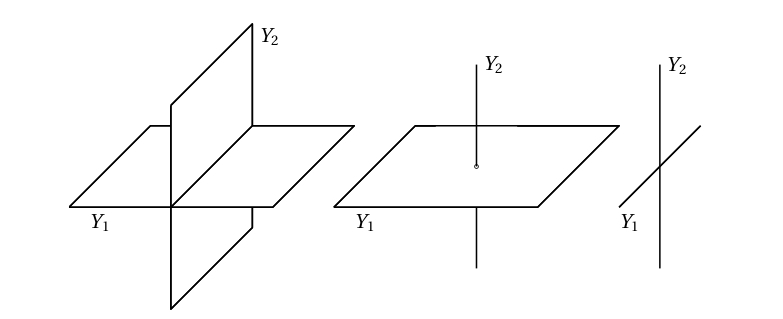
\includegraphics[scale=0.4]{2-5-1.jpg}
\end{center}
\subsubsection{Beispiel} 
Im Raum $X=\mathbb{R}^3$ ist die Gerade $Y_2:=\left\{\begin{pmatrix}x_1\\x_2\\x_3\end{pmatrix}\in X: x_1=x_2=x_3\right\}$ ein Komplement zur Ebene $Y_1:=\{x\in X: x_1-x_2+x_3=0\}$.\\
In der Tat liegt $x\in Y_1 \cap Y_2$, so erfüllen die Elemente des Durchschnitts\\
\[x_1-x_2+x_3=0\]
\[x_1-x_2=0\]
\[x_2-x_3=0\]
und folglich $x=0$, dies bedeutet $Y_1\cap Y_2=\{0\}$. Andererseits liegen $y_1=\begin{pmatrix}1\\1\\0\end{pmatrix}$, $y_2=\begin{pmatrix}1\\0\\-1\end{pmatrix}$ in $Y_1$ und $y_3=\begin{pmatrix}1\\1\\1\end{pmatrix}$ in $Y_2$. Da $\{y_1,y_2,y_3\}$ eine Basis von $\mathbb{R}^3=X$ bilden, gilt auch $Y_1+Y_2=X$.
\subsubsection{Beispiel}
Wir betrachten den Unterraum $Y_1:=\{p\in P(\mathbb{K}):p(0)=0\}$ von $X=P(\mathbb{K})$.  Dann gilt $P(\mathbb{K})=Y_1 \oplus P_0(\mathbb{K})$, d.h. der lineare Raum aller konstanten Polynome ist ein Komplement von $Y_1$.
\subsubsection{Satz}
Es seien $Y_1,Y_2\subseteq X$ Unterräume.  Es ist $X=Y_1\oplus Y_2$ genau dann, wenn es zu jedem $x\in X$ eindeutige $y_1\in Y_1,y_2\in Y_2$ mit $x=y_1+y_2$ gilt.\\
\underline{Beweis}:\\
($\Rightarrow$) Es sei $Y_2$ ein Komplement von $Y_1$ in $X$.  Wegen $Y_1+Y_2=X$ lässt sich jedes $x\in X$ darstellen als $x=y_1+y_2$ mit $y_1\in Y_1,y_2\in Y_2$.  Um deren Eindeutigkeit zu verifizieren, sein $\hat{y}_1\in Y_1,\hat{y}_2\in X_2$ zwei weitere Vektoren mit $x=\hat{y}_1+\hat{y}_2$.  Dies impliziert $y_1-\hat{y}_2=\hat{y}_2-y_2$ und $y_1-\hat{y}_1\in Y_1$ für $i=1,2$ und folglich $y_i-\hat{y}_i\in Y_1\cap Y_2$ für $i=1,2$.  Wegen $Y_1\cap Y_2 = \{0\}$ folgt $y_1=\hat{y}_1$ und $y_2=\hat{y}_2$.\\
\\
($\Leftarrow$) Umgekehrt seien $Y_1,Y_2\subseteq X$ Unterräume derart, dass sich jedes $x\in X$ eindeutig als Summe $X=y_1+y_2$ mit $y_i\in Y_i,i=1,2$, darstellen lässt.  Dann gilt sicherlich $Y_1+Y_2=X$.  Ist nun $x\in Y_1\cap Y_2$, so gilt $x=x+0=0+x$ und da die Darstellung eindeutig sein muss, resultiert $x=0;$ also $Y_1\cap Y_2=\{0\}$.
\subsubsection{Satz}
Jeder Unterraum eines endlich dimensionalen linearen Raumes hat ein Komplement.\\
\underline{Beweis}(-skizze):\\
Ergänze eine Basis von $Y_1$ zu einer Basis von $X$ gemäß \hyperref[2.4.9]{Proposition \ref*{2.4.9}}.
\subsection{Anwendung: Matrizen und lineare Gleichungen}
Es sei $\mathbb{K}$ ein Körper und $A\in\mathbb{K}^{m\times n}$ mit den $n$ Spalten und den $m$ Zeilen.  Die $n$ Spalten seien $a_1,\cdots ,a_n\in \mathbb{K}^m$ und $a^1,\cdots ,a^m\in \mathbb{K}^{1\times n}$ die Zeilen von $A$.  Man bezeichnet den Unterraum span$\{a_k\}_{1\leq k\leq n}\subseteq \mathbb{K}^m$ als Spaltenraum und span$\{a^1,\cdots ,a^m\}\subseteq \mathbb{K}^{1\times n}$ als \underline{Zeilenraum} von $A$.
\[A=\begin{pmatrix}a^1\\ \vdots \\ a^m\end{pmatrix} = (a_1,\cdots ,a_n)\]
\subsubsection{Definition (Rang einer Matrix)}
\label{Mrang}
Der \underline{Rang} (rk$A$) einer Matrix $A\in\mathbb{K}^{m\times n}$ ist die Dimension ihres Zeilenraumes.
\subsubsection{Bemerkung}
$0\leq$rk$A\leq m$
\[(L_0) Ax=0\]
\subsubsection{Proposition}
\label{2.6.3}
Der Lösungsraum $L_0\subseteq\mathbb{K}^n$ von ($L_0$) erfüllt dim$L_0=n-$rk$A$.\\
\underline{Beweis}:\\
Wir können o.B.d.A (ohne Beschränkung der Allgemeinheit) annehmen, dass $A\in\mathbb{K}^{m\times n}$ in strenger Zeilen-Stufen-Form ist.  Es sei $r$ die Anzahl der Zeilen von $A$, welche mindestens ein Element $\not=\ 0$ besitzen - dies ist der Rang von $A$.  Für $1\leq i\leq r$ sei $j_i$ derjenige Spaltenindex, in welcher das erste Element $\not=\ 0$ der $i$-ten Zeile steht.  Weiter seien $k_1,\cdots ,k_{n-r}$ diejenigen Element von $\{1,\cdots ,n\}$, welche nicht in $\{j_1,\cdots ,j_r\}$ sind.  Dann gilt 
\[L_0=\left\{x=\begin{pmatrix}\xi _1\\ \vdots \\ \xi_n\end{pmatrix}\in\mathbb{K}^n:\xi _1,\cdots ,\xi _{k_{n-r}} \in\mathbb{K}\ \mathrm{und}\ \xi _{j_i}=-\frac{1}{a_{i,j_i}}\sum_{j=1}^{n-r} a_{i,k_j} \xi _{k_j}\text{ für }1\leq i\leq r\right\}\]
und $x_1,\cdots x_{n-r}\in\mathbb{K}^n$ bezeichne die Vektoren in $L_0$ mit $\xi _{k_j}=1$ und $\xi _{k_i}=0$ für $i\not= j$.  Man überlegt sich nun, dass $\{x_1,\cdots x_{n-r}\}$ eine Basis von $L_0$ und die Behauptung folgt.
